\documentclass[tikz,border=10pt]{standalone}
\usepackage{amsmath} % For \text command
\usetikzlibrary{arrows.meta, positioning, fit, backgrounds}

\begin{document}

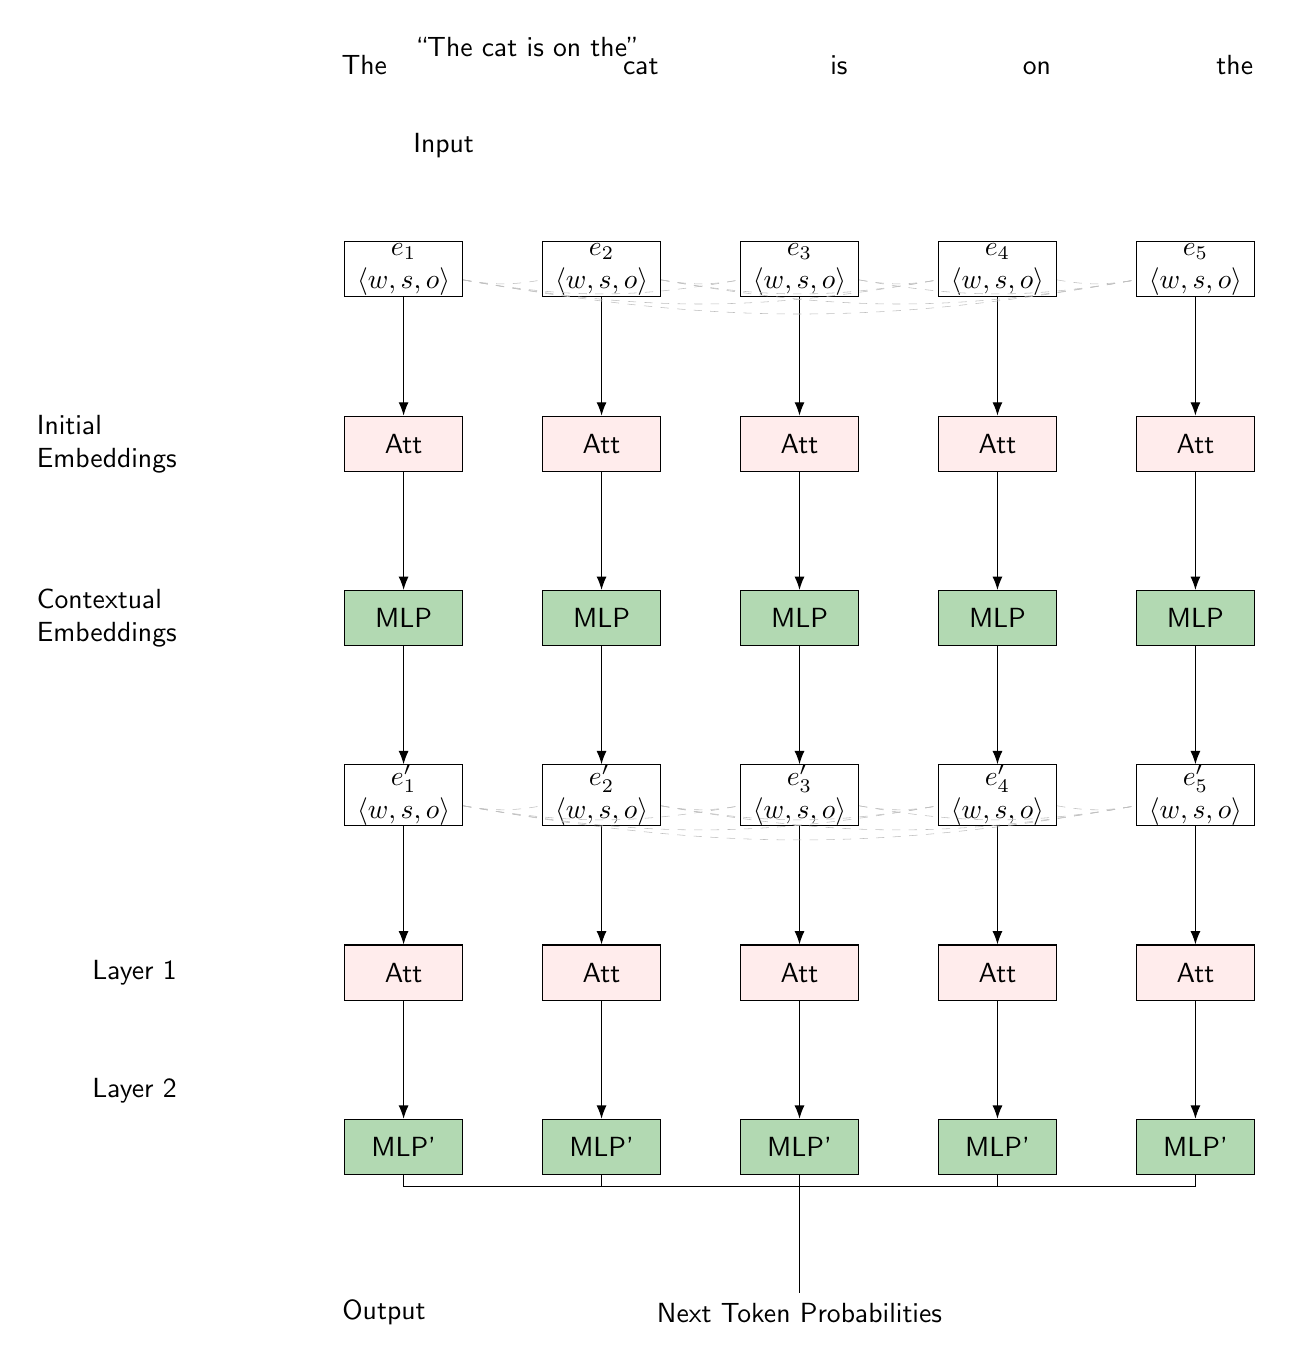
\begin{tikzpicture}[
    node distance = 1.5cm and 1cm,
    every edge/.append style = {draw, -Latex},
    font=\sffamily,
    >=Stealth,
    block/.style={rectangle, draw, fill=#1!30, minimum width=1.5cm, minimum height=0.7cm, align=center},
    attention/.style={block=pink, text width=1.2cm, text centered},
    mlp/.style={block=green!50!black, text width=1.2cm, text centered},
    embed/.style={block=white, text width=1.2cm, text centered, inner sep=0pt},
    dashed connection/.style={dashed, gray!50, bend right=10, very thin},
]

% Initial Embeddings
\node [embed] (e1) at (0,0) {$e_1$ \\ $\langle w, s, o \rangle$};
\node [embed, right=of e1] (e2) {$e_2$ \\ $\langle w, s, o \rangle$};
\node [embed, right=of e2] (e3) {$e_3$ \\ $\langle w, s, o \rangle$};
\node [embed, right=of e3] (e4) {$e_4$ \\ $\langle w, s, o \rangle$};
\node [embed, right=of e4] (e5) {$e_5$ \\ $\langle w, s, o \rangle$};

% Attention Layer 1
\node [attention, below=of e1] (att1_1) {Att};
\node [attention, below=of e2] (att1_2) {Att};
\node [attention, below=of e3] (att1_3) {Att};
\node [attention, below=of e4] (att1_4) {Att};
\node [attention, below=of e5] (att1_5) {Att};

% MLP Layer 1
\node [mlp, below=of att1_1] (mlp1_1) {MLP};
\node [mlp, below=of att1_2] (mlp1_2) {MLP};
\node [mlp, below=of att1_3] (mlp1_3) {MLP};
\node [mlp, below=of att1_4] (mlp1_4) {MLP};
\node [mlp, below=of att1_5] (mlp1_5) {MLP};

% Contextual Embeddings
\node [embed, below=of mlp1_1] (e1_prime) {$e_1'$ \\ $\langle w, s, o \rangle$};
\node [embed, below=of mlp1_2] (e2_prime) {$e_2'$ \\ $\langle w, s, o \rangle$};
\node [embed, below=of mlp1_3] (e3_prime) {$e_3'$ \\ $\langle w, s, o \rangle$};
\node [embed, below=of mlp1_4] (e4_prime) {$e_4'$ \\ $\langle w, s, o \rangle$};
\node [embed, below=of mlp1_5] (e5_prime) {$e_5'$ \\ $\langle w, s, o \rangle$};

% Attention Layer 2
\node [attention, below=of e1_prime] (att2_1) {Att};
\node [attention, below=of e2_prime] (att2_2) {Att};
\node [attention, below=of e3_prime] (att2_3) {Att};
\node [attention, below=of e4_prime] (att2_4) {Att};
\node [attention, below=of e5_prime] (att2_5) {Att};

% MLP Layer 2
\node [mlp, below=of att2_1] (mlp2_1) {MLP'};
\node [mlp, below=of att2_2] (mlp2_2) {MLP'};
\node [mlp, below=of att2_3] (mlp2_3) {MLP'};
\node [mlp, below=of att2_4] (mlp2_4) {MLP'};
\node [mlp, below=of att2_5] (mlp2_5) {MLP'};

% Next Token Probabilities
\node [below=1.5cm of mlp2_3, text width=5cm, align=center] (output) {Next Token Probabilities};

% Connections
\foreach \i in {1,...,5} {
    \draw (e\i) edge (att1_\i);
    \draw (att1_\i) edge (mlp1_\i);
    \draw (mlp1_\i) edge (e\i_prime);
    \draw (e\i_prime) edge (att2_\i);
    \draw (att2_\i) edge (mlp2_\i);
}

\draw (mlp2_1) --++ (0,-0.5) -| (output);
\draw (mlp2_2) --++ (0,-0.5) -| (output);
\draw (mlp2_3) --++ (0,-0.5) -| (output);
\draw (mlp2_4) --++ (0,-0.5) -| (output);
\draw (mlp2_5) --++ (0,-0.5) -| (output);

% Dashed connections for attention
\foreach \i/\j in {1/2, 1/3, 1/4, 1/5, 2/3, 2/4, 2/5, 3/4, 3/5, 4/5} {
    \draw[dashed connection] (e\i) to (e\j);
    \draw[dashed connection] (e\i_prime) to (e\j_prime);
}

% Labels
\node [above=of e1, anchor=north west] (input_label) {Input};
\node [above=of input_label.west, anchor=north west] {``The cat is on the''};

\node [left=of att1_1, xshift=-1cm, align=left] {Initial\\Embeddings};
\node [left=of att2_1, xshift=-1cm, align=left] {Layer 1};
\node [left=of mlp1_1, xshift=-1cm, align=left] {Contextual\\Embeddings};
\node [left=of att2_1, xshift=-1cm, yshift=-1.5cm, align=left] {Layer 2};
\node [left=of output, xshift=-1cm, align=left] {Output};

% Input words above initial embeddings
\node [above=of e1, xshift=-0.5cm, yshift=0.5cm] (word1) {The};
\node [above=of e2, xshift=0.5cm, yshift=0.5cm] (word2) {cat};
\node [above=of e3, xshift=0.5cm, yshift=0.5cm] (word3) {is};
\node [above=of e4, xshift=0.5cm, yshift=0.5cm] (word4) {on};
\node [above=of e5, xshift=0.5cm, yshift=0.5cm] (word5) {the};

\end{tikzpicture}

\end{document}